\documentclass{scrartcl}

\usepackage{fullpage}
\usepackage[utf8]{inputenc}
\usepackage{hyperref}
\usepackage{float}
%\usepackage[toc,page]{appendix}
\usepackage{tikz}
\usetikzlibrary{positioning}

\title{Report Generator}
\subtitle{module for otu.lea}
\author{Tamás Nagy\\ \small nattomi@gmail.com}

\begin{document}
\maketitle
\tableofcontents
\section{Introduction}
\href{http://github.com/nattomi/otulear}{Report Generator} is a module of the more complex \href{http://workforce.zmml.uni-bremen.de}{otu.lea} project. It is used for generating plain text and pdf reports about the performance of the users of the main \href{http://www.ifeb.uni-bremen.de/otulea/reaApplication.html}{otulea} test-taking application. It is a collection of \href{http://github.com/nattomi/otulear/tree/master/scripts}{scripts} (written in R and PHP) and \LaTeX\ templates. Additionally, routines used in the above mentioned scripts are also wrapped into an \href{http://github.com/nattomi/otulear/tree/master/otulea}{R package}. Momentarily it is not clear weather the R package is of any use, so its develepment is inactive. 

\section{How report generation works?}
Report generation is a process consisting of the following steps:
\begin{enumerate}
\item Load content of input data sources (such as .xml files) into memory
\item Extract information to be reported
\item\label{organ} Organize information to be reported into a structured form (such as .xml or .tex files)
\item If needed, run an external program (such as pdflatex) to translate the output of \ref{organ} into a human-readable form. 
\end{enumerate}
\begin{figure}[t]
\begin{center}
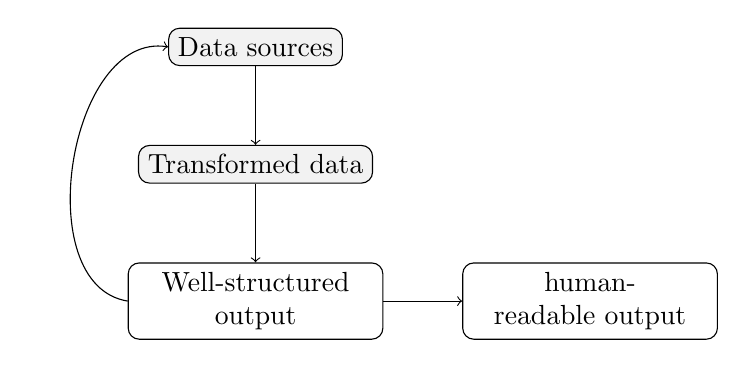
\begin{tikzpicture}[
mynode/.style={draw,fill=gray!10,rounded corners,align=center},
output/.style={draw,rounded corners,align=center}
]
\node[mynode] (sources) at (0,0) {Data sources};
\node[mynode, below=of sources] (trans) {Transformed data};
\node[output, below=of trans,text width=3cm] (struct) {Well-structured output};
\node[output,right=of struct,text width=3cm] (human) {human-readable output};
\draw[->] (sources) -- (trans);
\draw[->] (trans) -- (struct);
\draw[->] (struct) -- (human);
\path[->] (struct) edge [bend left=90] (sources);
\end{tikzpicture}
\end{center}
\caption{Simplified flow chart of report generation. It might be the case that a well-structured output of the report generation process becomes an input data source in a later stage.
}
\end{figure}
As an example, let's consider a speacial way to interpret the data generated by users of the otu.lea system, the so-called \emph{student report}. Here, we load certain .xml files, do some calculations on them according to some rules and dump the results of our calculations as an .xml file again. This .xml file is already an becomes the input of a new calculation stream which outputs a .tex file. This file is then rendered into a pdf file using pdflatex. We talk about this later in more detail.

In general, we can say that there is always some sort of database (either a relational one our a database of static files in a well-organized folder hierarchy just like in the case of otu.lea) we get our data from. We can think of report generation as if it were a certain \emph{view} to our database -- similar to the concept under the same name in database theory.

\section{The otu.lea database}
The database behind the otu.lea system is a collection of static .xml files. There are two main parts of this database. Files in the first part are for configuration purposes that only administrators can modify. From these, Report Generator only uses one file named \emph{alphalist.xml}. Files in the other part of the database are generated while users of the system are taking test-sessions. We use the term \emph{user files} to describe them.
\subsection{The alphalist.xml file}
\begin{figure}
\begin{center}
\begin{tikzpicture}[
mynode/.style={draw,fill=gray!10,rounded corners,align=center},
output/.style={draw,rounded corners,align=center,anchor=north}
]
\node[mynode] (root) at (0,0) {alphalist};
\node[output,anchor=north] (a1) at (-5,-1) {\parbox{2.6cm}{\textbf{alphanode}\\
\small{$\bullet$ alphaID\\
$\bullet$ order\\
$\bullet$ description\\
$\bullet$ userdescription\\
$\bullet$ example}}};
\node[output] (a2) at (-.5,-1) {\textbf{alphanode}};
\node[anchor=north] (a3) at (1.25,-1.1) {$\ldots$};
\node[output] (a4) at (3,-1) {\textbf{alphanode}};
\draw[--] (root) -- (a1);
\draw[--] (root) -- (a2);
\draw[--] (root) -- (a4);
\end{tikzpicture}
\end{center}
\caption{Tree structure of the alphalist.xml file. Each alphanode entry has 5 attributes.}
\label{fig:alphalist}
\end{figure}
The structure of the file is explained in Figure \ref{fig:alphalist}. It consists of multiple alphanode nodes. Each alphanode node has 5 attributes:
\begin{description}
\item[alphaID]: ability description ID.
\item[order]: unrelevant for Report Generator.
\item[description]: ability description displayed for teachers
\item[userdescription]: ability description displayed for students 
\item[example]: example clarifying ability description (to be shown to students)
\end{description}
Here is a snippet from the file:
\begin{verbatim}
<alphalist lang="german">
  <alphanode alphaID="1.2.1.2" order="60"
             description="Kann Zeitpläne sinnentnehmend lesen" 
             userdescription="Ich kann Zeitpläne lesen" example=""/>
 <alphanode alphaID="1.2.1.1" order="50" 
            description="Kann Wörter mit ansteigender Komplexität 
                        (Konsonantenhäufung) recodieren und decodieren" 
            userdescription="Ich kann einfache Wörter erkennen und lesen" 
            example=""/>
\end{verbatim}
\quad$\vdots$
\subsection{The user files}
There are two type of users of the otu.lea system: teachers and students. In this document -- if not otherwise stated -- by the term user we always mean students. Each user has an id which is a character string of a fixed length. Let's denote it by \verb+$userid+. Each user has a folder in the database named as \verb+$userid+. In each folder, there is a special file named \verb+$userid . ".xml"+ (we use the operator . for string concatenation as in PHP). This file describes the tests taken by the user, we call it the \emph{global user file}. It serves as a search index for finding the information related to any particular test a user has taken. From it we can determine:
\begin{itemize}
\item The date and time a partical test session was started
\item The subject and level of this particular test
\item The tasks contained by this particular test and the \emph{task-result files} linked to them
\end{itemize}
\begin{figure}
\begin{center}
\begin{tikzpicture}[
mynode/.style={draw,fill=gray!10,rounded corners,align=center},
output/.style={draw,rounded corners,align=center,anchor=north}
]
\node[mynode] (root) at (0,0) {performedtests};
\node[output,anchor=north] (a1) at (-5,-1) {\parbox{2.6cm}{\textbf{test}\\
\small{$\bullet$ timestamp\\
$\bullet$ subject\\
$\bullet$ level}}};
\node[output] (a2) at (-.5,-1) {\textbf{test}};
\node[anchor=north] (a3) at (1.25,-1.1) {$\ldots$};
\node[output] (a4) at (3,-1) {\textbf{test}};
\draw[--] (root) -- (a1);
\draw[--] (root) -- (a2);
\draw[--] (root) -- (a4);
\node[output,anchor=north] (i1) at (-10,-4) {\parbox{2.6cm}{\textbf{item}\\
\small{$\bullet$ iname\\
$\bullet$ data}}};
\node[output] (i2) at (-5.5,-4) {\textbf{item}};
\node[anchor=north] (i3) at (-3.75,-4.1) {$\ldots$};
\node[output] (i4) at (-2,-4) {\textbf{item}};
\draw[--] (a1) -- (i1);
\draw[--] (a1) -- (i2);
\draw[--] (a1) -- (i4);
\end{tikzpicture}
\end{center}
\caption{Tree structure of the global user file. It contains information about the performed tests and the tasks within those tests.}
\label{fig:guf}
\end{figure}
Figure \ref{fig:guf} shows the tree structure of the global user file. The main document consists of various \emph{test} nodes. Each test node has the follwing attributes:
\begin{description}
\item[timestamp] character string describing the date and time of the beginning of the test-session in the form of \verb+%Y_%m_%d_%H_%M_%S+ (see Appendix \ref{app:posix} for notation).
\item[subject] character string describing the subject of the test. It can be one of ``Lesen'', ``Schreiben'', ``Sprache'', ``Mathe''.
\item[level] character string describing the difficulty of the test. It can be one of ``Einfach'', ``Mittel'' and ``Schwer''. 
\end{description}
Furthermore, each test node has child nodes called \emph{item}. The attributes of each of these item nodes are in one-to-one correspondence with a task of the test the parent node referring to. It has the following attributes:
\begin{description}
\item[iname] character string describing the number of the task. The numbering convention of the tasks is not detailed here.
\item[data] character string describing the name of the task-result file. The task-result files of a user are located in the same folder as the global user file. 
\end{description}
Below is a snippet from a global user file:
\begin{verbatim}  
<performedtests>
  <test timestamp="2014_2_27_12_40_49" subject="Schreiben" level="Einfach">
    <item iname="2.1.01" data="KFCG1_2014_2_27_12_40_49_2.1.01.xml"/>
    <item iname="2.1.02_I" data="KFCG1_2014_2_27_12_43_37_2.1.02_I.xml"/>
    <item iname="2.1.02_II" data="KFCG1_2014_2_27_12_47_9_2.1.02_II.xml"/>
    <item iname="2.2.01_III" data="KFCG1_2014_2_27_12_48_53_2.2.01_III.xml"/>
    <item iname="2.2.02_I" data="KFCG1_2014_2_27_12_52_11_2.2.02_I.xml"/>
  </test>
  <test timestamp="2014_2_27_18_37_23" subject="Lesen" level="Mittel">
    <item iname="1.3.2" data="KFCG1_2014_2_27_18_37_23_1.3.2.xml"/>
    <item iname="1.3.3" data="KFCG1_2014_2_27_18_40_45_1.3.3.xml"/>
    <item iname="1.3.4" data="KFCG1_2014_2_27_18_42_27_1.3.4.xml"/>
    <item iname="1.3.6" data="KFCG1_2014_2_27_18_43_53_1.3.6.xml"/>
    <item iname="1.4.1" data="KFCG1_2014_2_27_19_11_28_1.4.1.xml"/>
    <item iname="1.4.2" data="KFCG1_2014_2_27_19_14_19_1.4.2.xml"/>
    <item iname="1.4.4" data="KFCG1_2014_2_27_19_18_7_1.4.4.xml"/>
    <item iname="1.4.5" data="KFCG1_2014_2_27_19_22_52_1.4.5.xml"/>
    <item iname="1.4.6" data="KFCG1_2014_2_27_19_25_18_1.4.6.xml"/>
    <item iname="1.4.7" data="KFCG1_2014_2_27_19_27_16_1.4.7.xml"/>
    <item iname="1.4.8" data="KFCG1_2014_2_27_19_29_40_1.4.8.xml"/>
  </test>
\end{verbatim}
\quad$\vdots$

The structure of the task-result files are more diverse, but as Report Generator only uses a specific segment of the file, we intruduce only this segment in Figure \ref{fig:taskresult}.
\begin{figure}
\begin{center}
\begin{tikzpicture}[
mynode/.style={draw,fill=gray!10,rounded corners,align=center},
output/.style={draw,rounded corners,align=center,anchor=north}
]
\node[mynode] (root) at (0,0) {item};
\node[output] (marking) at (0,-1) {marking};
\node[output] (pointuse) at (-7,-2.5) {pointuse};
\node[output] (m1) at (-3.5,-2.5) {\parbox{2.6cm}{\textbf{mark}\\
\small{$\bullet$ itemnumber\\
$\bullet$ alphalevel}}};
\node[output] (m2) at (-.5,-2.5) {\textbf{mark}};
\node at (.75,-2.75) {$\ldots$};
\node[output] (m3) at (2,-2.5) {\textbf{mark}};
\draw[--] (root) -- (marking);
\draw[--] (marking) -- (pointuse);
\draw[--] (marking) -- (m1);
\draw[--] (marking) -- (m2);
\draw[--] (marking) -- (m3);
\end{tikzpicture}
\end{center}
\caption{Tree structure of the segment of the task-result file relevant to Report Generator.}
\label{fig:taskresult}
\end{figure}
In the task-result files there is always a \emph{marking} node whose children nodes we are interested in. It always has a child node named \emph{pointuse} which is not relevant to our calculations so we omit describing it. Its other children nodes are all named \emph{mark} and they describe the performance of the user on a subtask of the task in question. Performance can be either 1 (passed) or 0 (failed). Each mark node has (at least) the following attributes:
\begin{description}
\item[itemnumber] character string describing the subtask number the mark node is referring to
\item[alphalevel] ability description id of the ability description which is tested by the mark node
\end{description} 
Below is the simplified version of a the task-result file showing only the nodes relevant to Report Generator.
\begin{verbatim}
<item>
  <marking>
    <pointuse maxpoint="1"/>
    <mark itemnumber="2.1.01_1a" alphalevel="2.1.05">1</mark>
    <mark itemnumber="2.1.01_1b" alphalevel="2.1.14">1</mark>
    <mark itemnumber="2.1.01_2a" alphalevel="2.1.05">1</mark>
    <mark itemnumber="2.1.01_2b" alphalevel="2.1.14">1</mark>
    <mark itemnumber="2.1.01_3a" alphalevel="2.1.05">1</mark>
    <mark itemnumber="2.1.01_3b" alphalevel="2.1.04">1</mark>
    <mark itemnumber="2.1.01_4a" alphalevel="2.1.05">1</mark>
    <mark itemnumber="2.1.01_4b" alphalevel="2.1.14">1</mark>
    <mark itemnumber="2.1.01_5a" alphalevel="2.1.05">1</mark>
    <mark itemnumber="2.1.01_5b" alphalevel="2.1.14">0</mark>
    <mark itemnumber="2.1.01_5c" alphalevel="2.1.14">0</mark>
  </marking>
</item>
\end{verbatim}

\section{Description of reports}
\subsection{Student report}
\subsection{Teacher report}
\subsection{DT type teacher report}
\appendix
\section{ISO C99 / POSIX standard for 'strftime'}\label{app:posix}
\begin{tabular}{rp{14cm}} 
\%d & Day of the month as decimal number (01-31).\\
\%H & Hours as decimal number (00-23).  As a special exception times such as ‘24:00:00’ are accepted for input, since ISO 8601 allows these.\\
\%m & Month as decimal number (01-12).\\
\%M & Minute as decimal number (00-59).\\
\%S & Second as decimal number (00-61), allowing for up to two leap-seconds (but POSIX-compliant implementations will ignore leap seconds).\\
\%Y & Year with century.  Note that whereas there was no zero in the original Gregorian calendar, ISO 8601:2004 defines it to be valid (interpreted as 1BC): see \url{http://en.wikipedia.org/wiki/0_(year)}.  Note that the standard also says that years before 1582 in its calendar should only be used with agreement of the parties involved.
\end{tabular}
\end{document}
